% Fig. 3: the memory limit (schematic). Width 7.05 in = 17.907 cm, height 6.55 cm.
% Panel a (fig3a.pdf, matplotlib, included at 100%): the limit versus k between the two bounds of Theorem 1, with the
% reservoirs of panel b on it and their levels W_{q,2} and W_{q,4}.
% Panel b (drawn here): one input stream u_t (a sine) drives three reservoirs, drawn as qubit lattices at the same
% lattice spacing: B (n = 100, k = 2) on top, A (n = 10, k = 2) in the middle, C (n = 10, k = 4) below, so that both
% comparisons start from A. Input qubits are purple. In each lane, the inputs within the limit are on blue (within
% reach; the curve fades as the influence of an input decays with its age), older inputs on red (out of reach for every
% reservoir with this k), separated by the red wall of the limit, as on the memory axis of Fig. 1(c). B and A share the
% limit W_{q,2}; two more input qubits move the wall from A to C, back to W_{q,4}.
\documentclass[border=0pt]{standalone}
% Shared TikZ style for the schematics. Same typeface, size (8 pt) and palette as figstyle.py:
% blue = memory / reservoir dynamics, red = noise and the limit, purple = input, greys = neutral.
\usepackage[T1]{fontenc}
\usepackage{helvet}
\renewcommand{\familydefault}{\sfdefault}
\usepackage{amsmath,amssymb,bm}
\usepackage{tikz}
\usetikzlibrary{arrows.meta,calc,decorations.pathreplacing,patterns.meta,shapes.geometric,shadows}
\definecolor{cInk}{HTML}{1A1A1A}
\definecolor{cBlue}{HTML}{3C7FE0}
\definecolor{cBlueDark}{HTML}{1D4C9C}
\definecolor{cBlueLight}{HTML}{8DB8F0}
\definecolor{cBlueFill}{HTML}{DDE9F9}
\definecolor{cRed}{HTML}{EF4B3B}
\definecolor{cRedDark}{HTML}{B8301F}
\definecolor{cRedFill}{HTML}{FCE3DE}
\definecolor{cPurple}{HTML}{9B4FE0}
\definecolor{cPurpleDark}{HTML}{6B2CAB}
\definecolor{cPurpleFill}{HTML}{EFE2FB}
\definecolor{cGreyDark}{HTML}{4A4A4A}
\definecolor{cGrey}{HTML}{8C8C8C}
\definecolor{cGreyLight}{HTML}{B4B4B4}
\definecolor{cGreyFill}{HTML}{EDEDED}
\definecolor{cShadow}{HTML}{B5B5B5}
\tikzset{
  every node/.style={font=\fontsize{8}{9.6}\selectfont},
  lbl/.style={font=\fontsize{8}{9.6}\selectfont},
  ttl/.style={font=\fontsize{8}{9.6}\selectfont,anchor=base west,inner sep=0pt},
  ttlr/.style={font=\fontsize{8}{9.6}\selectfont,anchor=base east,inner sep=0pt},
  wire/.style={line width=0.65pt,cInk},
  ublk/.style={draw=cInk,line width=0.6pt,fill=cBlue,rounded corners=1.6pt},
  iblk/.style={draw=cInk,line width=0.6pt,rounded corners=1.6pt,preaction={fill=cPurple},
    pattern={Lines[angle=55,distance=2.2pt,line width=0.85pt]},pattern color=white},
  nbox/.style={draw=cInk,line width=0.55pt,fill=cRed,rounded corners=1.1pt},
  feat/.style={draw=cInk,line width=0.6pt,fill=white,rounded corners=2pt,inner sep=1.6pt,
    minimum width=0.98cm,minimum height=0.44cm},
  legbox/.style={draw=cInk,line width=0.8pt,fill=white,rounded corners=2.4pt,
    drop shadow={shadow xshift=1.2pt,shadow yshift=-1.2pt,fill=cShadow,opacity=1}},
  arr/.style={line width=0.65pt,-{Stealth[length=3.6pt,width=3.2pt]}},
  brc/.style={decorate,decoration={brace,amplitude=2.6pt},line width=0.55pt},
}
\newcommand{\Discard}[3][cInk]{%
  \draw[line width=0.75pt,#1] (#2,{#3-0.1}) -- (#2,{#3+0.1});
  \draw[line width=0.75pt,#1] ({#2+0.05},{#3-0.064}) -- ({#2+0.05},{#3+0.064});
  \draw[line width=0.75pt,#1] ({#2+0.1},{#3-0.03}) -- ({#2+0.1},{#3+0.03});}
\providecommand{\ket}[1]{|#1\rangle}
\providecommand{\nrm}[2]{\lvert #1\rvert_{#2}}

\usetikzlibrary{shadows.blur}
\begin{document}
\begin{tikzpicture}[x=1cm,y=1cm]
\def\H{6.55}
\useasboundingbox (0,0) rectangle (17.907,\H);
\node[anchor=north west,inner sep=0pt,outer sep=0pt] at (0,\H) {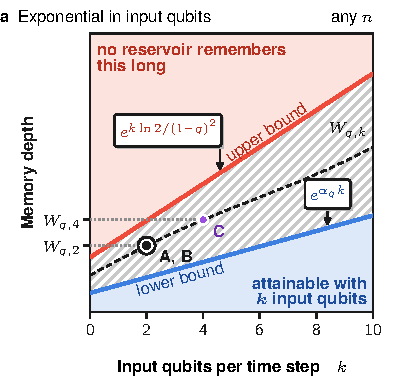
\includegraphics{fig3a.pdf}};
% =================================================================================== panel b
\def\XB{7.15}% left edge of panel b
\node[ttl] at (\XB,{\H-0.367}) {\textbf{b}\enspace Input qubits, not size, set the limit};
% ------------------------------------------------------------------ geometry
\def\xL{8.89}\def\xT{12.99}\def\xE{13.17}% track: start, present (time t), rounded end
\def\hT{0.33}% half height of a track
\def\wTwo{11.39}\def\wFour{9.44}% walls: t - W_{q,2} and t - W_{q,4}
\def\yB{5.05}\def\yA{3.60}\def\yC{2.00}% lane centres: B on top, A in the middle, C below
\def\amp{0.19}% amplitude of the input curve
\def\uT{0.149}% value of the curve at time t (cm above the lane centre)
\def\xP{14.00}% left-corner qubit of every reservoir
% the input stream, a sine with 5.5 periods along the track that ends at time t on a rising flank
\newcommand{\Curve}[1]{plot[domain=0:1,samples=181]
  ({\xL+0.06+(\xT-\xL-0.06)*\x},{#1+\amp*sin(deg(2*pi*5.5*(\x-1)+0.9))})}
% ------------------------------------------------------------------ a lane: track, input curve, wall, current input
% #1 lane centre, #2 wall position
\newcommand{\Lane}[2]{%
  \begin{scope}
    \clip[rounded corners=0.13cm] (\xL,{#1-\hT}) rectangle (\xE,{#1+\hT});
    \fill[cRedFill] (\xL,{#1-\hT}) rectangle (#2,{#1+\hT});
    \fill[cBlueFill] (#2,{#1-\hT}) rectangle (\xE,{#1+\hT});
    \begin{scope}\clip (\xL,{#1-1}) rectangle (#2,{#1+1});
      \draw[cGreyLight,line width=0.9pt,line join=round] \Curve{#1};
    \end{scope}
    % within reach: the curve fades from the present (black) towards the limit, as the influence of an input
    % decays with its age
    \foreach \s in {0,...,11} {
      \pgfmathsetmacro\xa{#2+(\xE-#2)*\s/12}\pgfmathsetmacro\xb{#2+(\xE-#2)*(\s+1)/12}
      \pgfmathtruncatemacro\fadeval{40+60*(\s+0.5)/12}
      \begin{scope}\clip (\xa,{#1-1}) rectangle ({\xb+0.002},{#1+1});
        \draw[cInk!\fadeval!cGreyLight,line width=0.9pt,line join=round] \Curve{#1};
      \end{scope}}
  \end{scope}
  \draw[cGrey,line width=0.6pt,rounded corners=0.13cm] (\xL,{#1-\hT}) rectangle (\xE,{#1+\hT});
  \draw[cRed,line width=2.0pt] (#2,{#1-\hT-0.07}) -- (#2,{#1+\hT+0.07});
  \fill[cPurple,draw=white,line width=0.5pt] (\xT,{#1+\uT}) circle[radius=0.062];}
% ------------------------------------------------------------------ a reservoir: qubit lattice on a plate (isometric)
% Lattice coordinates (i,j): i runs along the front-left edge (down to the right), j along the front-right edge (up to
% the right); the left corner of the plate faces the lanes. #1,#2 left-corner qubit; #3 qubits along i; #4 qubits
% along j; #5 input qubits (purple, along the front-left edge from the left corner).
\def\La{0.205}\def\rq{0.083}\def\Lm{0.78}\def\Lh{0.085}
\newcommand{\Plate}[5]{%
  \pgfmathsetmacro\iE{#3-1+\Lm}\pgfmathsetmacro\jE{#4-1+\Lm}%
  \pgfmathtruncatemacro\nC{#3-1}\pgfmathtruncatemacro\nR{#4-1}%
  \pgfmathsetmacro\kE{#5-1+0.56}%
  \begin{scope}[shift={(#1,#2)},x={({\La*0.866cm},{-\La*0.5cm})},y={({\La*0.866cm},{\La*0.5cm})}]
    % soft shadow, slab (thickness) and top face, with rounded corners
    \fill[blur shadow={shadow xshift=1.4pt,shadow yshift=-3.2pt,shadow blur radius=3.2pt,shadow opacity=45},
      cGreyLight,rounded corners=1.8pt] ([yshift=-\Lh cm]-\Lm,-\Lm) -- ([yshift=-\Lh cm]\iE,-\Lm)
      -- ([yshift=-\Lh cm]\iE,\jE) -- ([yshift=-\Lh cm]-\Lm,\jE) -- cycle;
    \foreach \t in {1,...,6} {
      \pgfmathsetmacro\dz{\t*\Lh/6}
      \fill[left color=cGreyFill,right color=cGreyLight,rounded corners=1.8pt]
        ([yshift=-\dz cm]-\Lm,-\Lm) -- ([yshift=-\dz cm]\iE,-\Lm) -- ([yshift=-\dz cm]\iE,\jE)
        -- ([yshift=-\dz cm]-\Lm,\jE) -- cycle;}
    \draw[cGreyLight!70!cGrey,line width=0.4pt,rounded corners=1.8pt]
      ([yshift=-\Lh cm]-\Lm,-\Lm) -- ([yshift=-\Lh cm]\iE,-\Lm) -- ([yshift=-\Lh cm]\iE,\jE);
    \shade[top color=white,bottom color=cGreyFill,draw=cGreyLight,line width=0.5pt,rounded corners=1.8pt]
      (-\Lm,-\Lm) -- (\iE,-\Lm) -- (\iE,\jE) -- (-\Lm,\jE) -- cycle;
    % input register: the input qubits on a purple field, as in Fig. 4(a)
    \filldraw[fill=cPurpleFill,draw=cPurple,line width=0.6pt,rounded corners=1.4pt]
      (-0.56,-0.56) -- (\kE,-0.56) -- (\kE,0.56) -- (-0.56,0.56) -- cycle;
    % couplings
    \foreach \j in {0,...,\nR} {
      \foreach \i in {0,...,\nC} {
        \ifnum\i<\nC\relax \draw[cGreyLight,line width=0.5pt] (\i,\j) -- ({\i+1},\j);\fi
        \ifnum\j<\nR\relax \draw[cGreyLight,line width=0.5pt] (\i,\j) -- (\i,{\j+1});\fi
      }}
    % qubits, from the back row to the front
    \foreach \j in {\nR,...,0} {
      \foreach \i in {0,...,\nC} {
        \pgfmathtruncatemacro\isin{(\j==0)&&(\i<#5)}
        \ifnum\isin=1 \shade[ball color=cPurple!80!white] (\i,\j) circle[radius=\rq cm];
        \else \shade[ball color=cBlue] (\i,\j) circle[radius=\rq cm];\fi
      }}
  \end{scope}}
% ------------------------------------------------------------------ the three lanes
\Lane{\yB}{\wTwo}
\Lane{\yA}{\wTwo}
\Lane{\yC}{\wFour}
\Plate{\xP}{\yB+0.20}{10}{10}{2}
\Plate{\xP}{\yA+0.10}{5}{2}{2}
\Plate{\xP}{\yC+0.10}{5}{2}{4}
% input stream into the input qubits
\foreach \y/\dy in {\yB/0.20,\yA/0.10,\yC/0.10}
  \draw[arr,cPurple,line width=0.8pt] ({\xT+0.08},{\y+\uT}) to[out=0,in=180] ({\xP-0.15},{\y+\dy});
% ------------------------------------------------------------------ labels of the lanes
\newcommand{\LaneLabel}[4]{% y, letter, line with n, line with k
  \node[anchor=base west,inner sep=0pt] at (\XB,{#1+0.04}) {\textbf{#2}};
  \node[anchor=base west,inner sep=0pt] at ({\XB+0.42},{#1+0.04}) {#3};
  \node[anchor=base west,inner sep=0pt] at ({\XB+0.42},{#1-0.32}) {#4};}
\LaneLabel{\yB}{B}{$\bm{n=100}$}{$k=2$}
\LaneLabel{\yA}{A}{$n=10$}{$k=2$}
\LaneLabel{\yC}{C}{$n=10$}{\textcolor{cPurpleDark}{$\bm{k=4}$}}
% region names above the top lane
\node[anchor=base east,inner sep=0pt,text=cRedDark] at ({\wTwo-0.14},{\yB+\hT+0.17}) {\textbf{out of reach, for any $\bm n$}};
\node[anchor=base west,inner sep=0pt,text=cBlueDark] at ({\wTwo+0.14},{\yB+\hT+0.17}) {\textbf{within reach}};
% same limit for B and A
\draw[cRed,line width=0.8pt,dash pattern=on 2.2pt off 1.6pt] (\wTwo,{\yB-\hT-0.07}) -- (\wTwo,{\yA+\hT+0.07});
\node[anchor=west,inner sep=0pt,text=cRedDark] at ({\wTwo+0.12},{(\yA+\yB)/2}) {same limit};
% two more input qubits move the wall from A to C
\draw[arr,cPurple,line width=1.0pt] (\wTwo,{\yA-\hT-0.09})
  .. controls (\wTwo,{\yA-\hT-0.62}) and (\wFour,{\yC+\hT+0.62}) .. (\wFour,{\yC+\hT+0.10});
\node[anchor=west,align=left,inner sep=0pt,text=cPurpleDark] at ({\wTwo+0.26},{(\yA+\yC)/2+0.02})
  {$+2$ input qubits:\\higher limit};
% ------------------------------------------------------------------ time axis
\def\yX{1.27}
\draw[line width=0.8pt,cInk] (\xL,\yX) -- (\xE,\yX);
\foreach \x/\l in {\wFour/{t-W_{q,4}},\wTwo/{t-W_{q,2}},\xT/{t}} {
  \draw[line width=0.8pt,cInk] (\x,\yX) -- (\x,{\yX-0.106});
  \node[anchor=north,inner sep=0pt] at (\x,{\yX-0.19}) {$\l$};}
\node[anchor=base,inner sep=0pt] at ({(\xL+\xE)/2},0.25) {\textbf{Time step}};
\end{tikzpicture}
\end{document}
